\documentclass{article}
\usepackage[utf8]{inputenc}
\usepackage{geometry}
\usepackage{graphicx}
\geometry{
	a4paper,
	total={155mm,242mm},
	inner=30mm,
	top=20mm,
}
\usepackage{hyperref}

\title{\textsc{CMlib} -- Cell mapping algorithms in \texttt{C++}}
\author{Gergely Gyebrószki$^1$ \\
$^1$: Dept. of Applied Mechanics, Budapest University of Technology and Economics}
\date{27. February, 2019}

\begin{document}
\maketitle

{\small The latest version of this document is available at: \href{https://github.com/Gyebro/cell-mapping/blob/master/docs/tex/cell-mapping-cpp.pdf}{github.com/Gyebro/cell-mapping}}
	
\section{Introduction and goals}

\section{Features}

\subsection{Cell mapping algorithms}

\subsection{Highlights of the C++ implementation}

\section{Documentation}

\subsection{Source code documentation}

\subsection{title}

\section{Installation}

\section{Examples}

\subsection{Simple pendulum}

\begin{figure}[h]
	\centering
	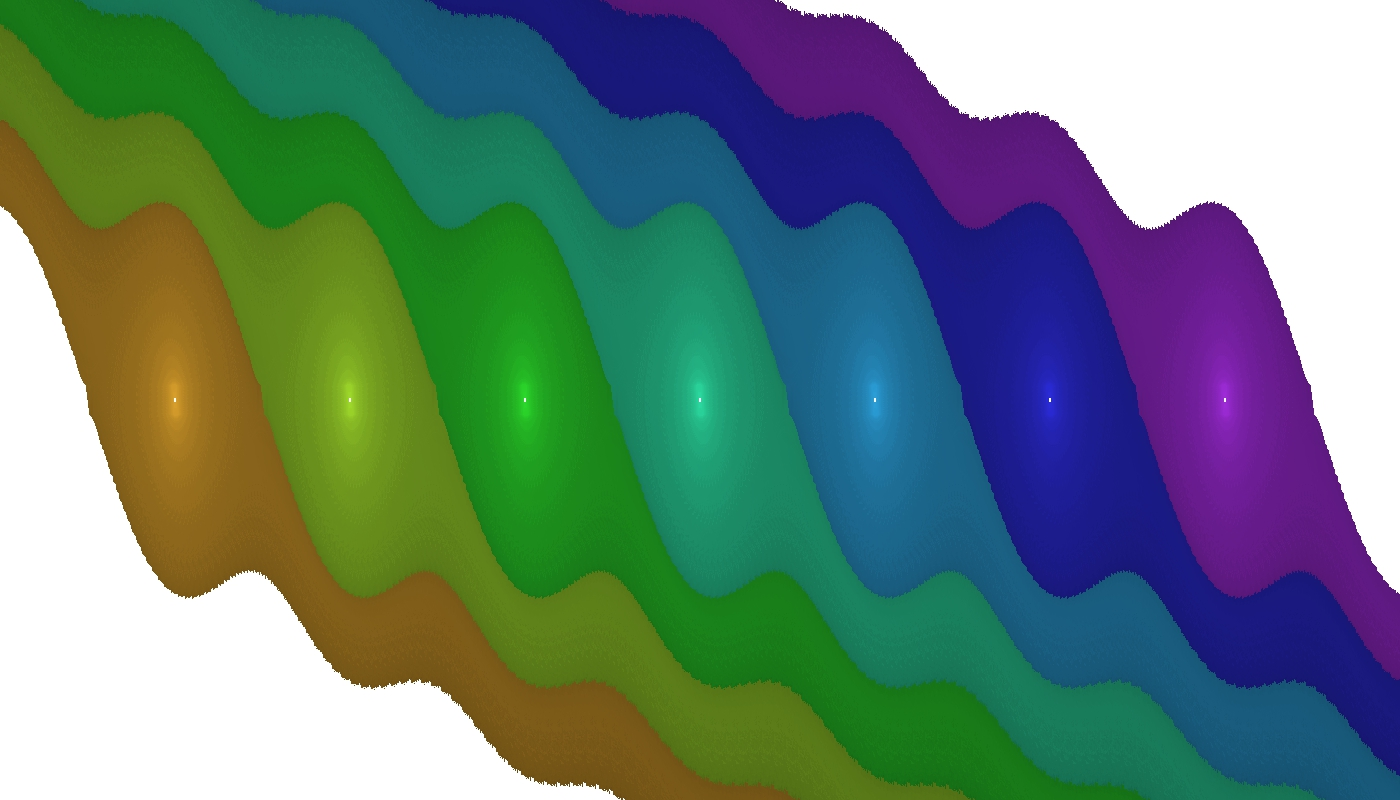
\includegraphics[width=12cm]{fig/pendulum.jpg}
	\caption{SCM results for the simple pendulum.}
\end{figure}


\subsection{Micro-chaos map}

\begin{figure}[h]
	\centering
	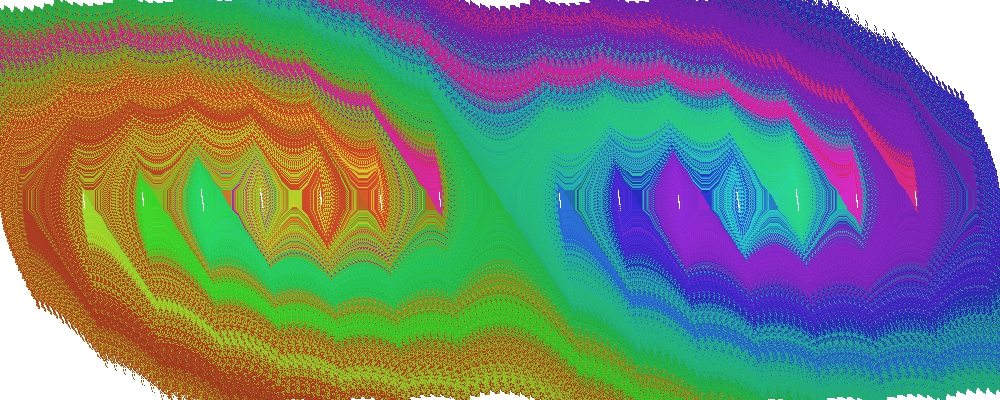
\includegraphics[width=12cm]{fig/microchaos.jpg}
	\caption{SCM results for the micro-chaos map.}
\end{figure}

\subsection{Duffing oscillator}

\begin{figure}[h]
	\centering
	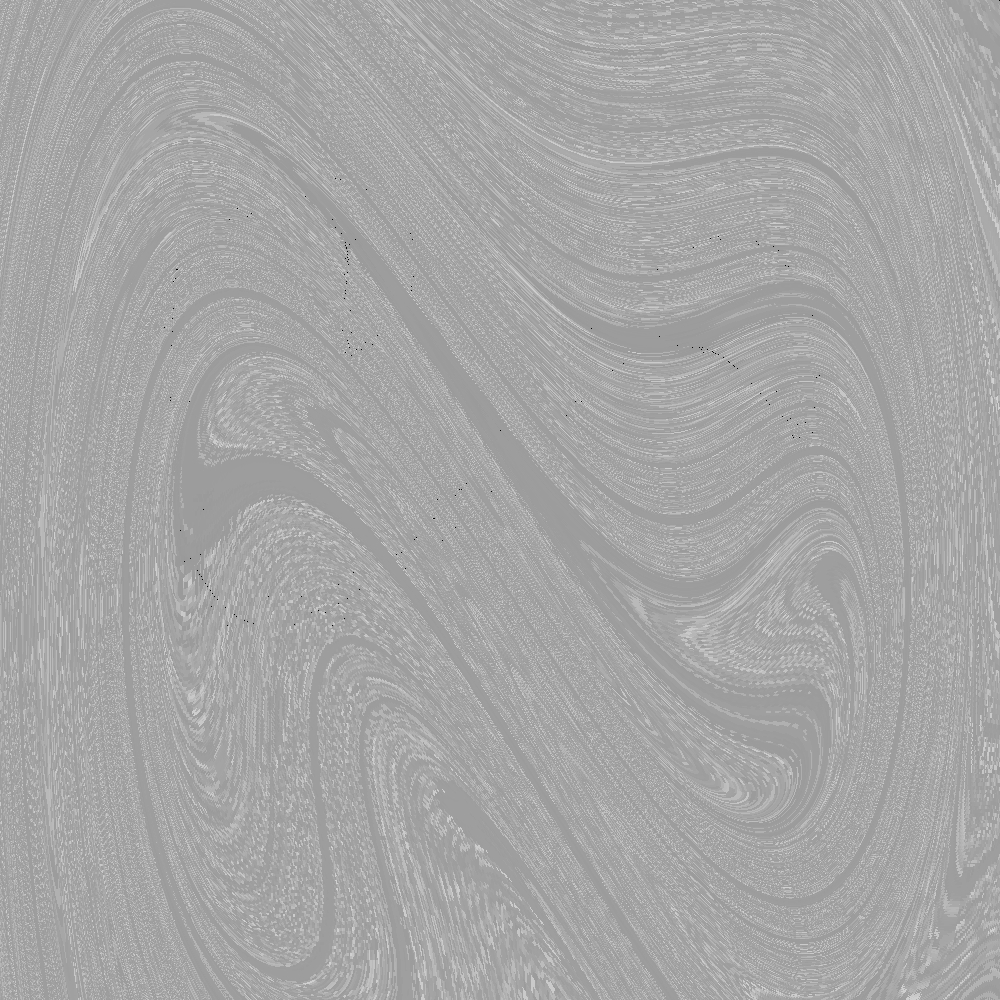
\includegraphics[width=10cm]{fig/duffing.jpg}
	\caption{SCM results for the Duffing oscillator Poincaré-section.}
\end{figure}

\end{document}